\chapter{球対称ポテンシャルと時間積分法}
\label{chap:orbits}

第1--2章では、球対称な密度分布から重力場を求めた。
本章では、同じ Plummer 球の重力場の中で星の位置と速度の時間変化を計算し、常微分方程式の時間積分法を学ぶ。
時間積分そのものの誤差を調べるため、加速度には解析式を用い、第2章の数値重力場に含まれる誤差とは切り分けて検証する。

運動方程式に初期位置と初期速度を与えると、その後の軌道を求める初期値問題となる。
Euler 法、古典的4次 Runge--Kutta 法（RK4）、リープフロッグ法（leapfrog method）を同じ軌道に適用し、時間刻みを変えた収束試験と保存量の変化から結果を検証する。
軌道の物理は Ryden §7.1\cite{ryden2025}、Euler 法と RK4 は幸谷 第13章\cite{kouya2021}、リープフロッグ法の長時間挙動は松本ほか §9.6\cite{matsumoto}を参照する。

\begin{learningbox}[本章で学ぶこと]
\begin{itemize}
 \item 運動方程式を、位置と速度を未知数とする1階の常微分方程式系に書き換え、初期値問題として設定できる。
 \item Euler 法、RK4、リープフロッグ法の更新の考え方を説明し、時間ループとして実装できる。
 \item 円軌道の解析解との比較と時間刻みを変えた収束試験から、時間積分法の誤差と収束次数を評価できる。
 \item エネルギーと角運動量の変化を用いて数値軌道を診断し、保存量だけでは位置の精度を判断できないことを説明できる。
 \item 収束次数と長時間積分での保存量の振る舞いを区別し、必要な精度・積分時間・計算コストに応じて時間積分法を選ぶ際の考え方を説明できる。
\end{itemize}
\end{learningbox}

本章の数値実験は Notebook 3 で行う。
本文では更新式と計算部分の対応を示し、完全な可視化コードは Notebook に置く。
軸対称・非軸対称の軌道は付録\ref{app:orbit-applications}で扱い、本章は球対称モデルだけで学習できる。
% =====================================================================
\section{Plummer 球の重力場と軌道計算の準備}
\label{sec:ch3-plummer}

第1--2章で用いた Plummer ポテンシャル
\begin{equation}
 \Phi(r)=-\frac{GM}{\sqrt{r^2+a^2}}
\label{eq:ch3-plummer-potential}
\end{equation}
の中で星の軌道を計算する。
重力場は時間に依存せず、計算する星の運動によっても変化しないものとする。
中心から測った位置ベクトルを $\boldsymbol{x}$、その大きさを $r=|\boldsymbol{x}|$ と書く。
第2章と同様に、動径方向の重力加速度を $g_r=-d\Phi/dr$ とする。
軌道計算では重力加速度をベクトルとして扱うため、以下では重力加速度ベクトルを $\boldsymbol{g}$ と書く。
球対称系では、中心以外で
\begin{equation}
 \boxed{\boldsymbol{g}=g_r\frac{\boldsymbol{x}}{r}=-\frac{GM}{(r^2+a^2)^{3/2}}\boldsymbol{x}}
\label{eq:ch3-plummer-acc}
\end{equation}
となる。この右辺は中心でもそのまま評価でき、$\boldsymbol{g}(\boldsymbol{0})=\boldsymbol{0}$ である。\footnote{
このポテンシャルは、無衝突系を扱う重力 $N$ 体計算で用いられる\textbf{Plummer 型ソフトニング（softening）}と同じ関数形を持つ\cite{matsumoto}。
粒子間距離を $r$、粒子質量を $m$ とし、ポテンシャルを $-Gm/\sqrt{r^2+\epsilon^2}$ とすると、$\epsilon>0$ なら $r\to0$ でも重力加速度は発散しない。
ただし、本章の $a$ は質量モデル全体のスケール半径であり、$\epsilon$ は粒子間の重力を平滑化する長さである。
同じ関数形に現れるが、両者の役割は異なる。
}

Notebook 3 では $G=M=a=1$ の無次元単位を用いる。
質量単位を $M$、長さ単位を $a$ とし、時間単位 $t_\ast$ を $a/t_\ast^2=GM/a^2$ となるように選ぶと、
\begin{equation}
 t_\ast=\sqrt{\frac{a^3}{GM}},\qquad
 v_\ast=\sqrt{\frac{GM}{a}},\qquad
 \Phi_\ast=\frac{GM}{a}
\label{eq:ch3-dynamical-units}
\end{equation}
を得る。
無次元の時刻・速度・ポテンシャルを物理単位へ戻すときは、それぞれ $t_\ast$、$v_\ast$、$\Phi_\ast$ を掛ければよい。

以下では、位置ベクトルから Plummer ポテンシャルと重力加速度を
計算する関数を定義する。

\begin{notebookblock}{3｜Plummer 球の重力場}
初期条件・解析解・軌道計算で同じ $G,M,a$ を使う。

\texttt{phi\_plummer\_pos} は、位置ベクトルからポテンシャルを計算する。
\texttt{np.sum(x**2, axis=-1)} は、位置ベクトルの各成分の二乗和を求める。
\texttt{axis=-1} は配列の最後の軸を指定しており、
複数の時刻の位置をまとめて与えた場合にも、それぞれのポテンシャルを計算できる。

\texttt{acc\_plummer} は、一つの位置ベクトルから重力加速度を計算する。
\texttt{acc\_plummer\_model} は、設定した $G,M,a$ を用いて、
位置ベクトルだけから加速度を計算する補助関数である。
後の時間積分では、この関数を使用する。

\par\smallskip\noindent\begin{minipage}{\linewidth}
{\sffamily\small\color{graytext}対応セル（重力場の定義）}
\begin{Verbatim}[xleftmargin=2mm,fontsize=\small,frame=single,framesep=1.8mm,framerule=0.35pt,rulecolor=\color{listingframe},fillcolor=\color{listingbg}]
import numpy as np

# 無次元単位を設定する
G = 1.0
M = 1.0
a = 1.0

# 位置ベクトルからPlummerポテンシャルを計算する
def phi_plummer_pos(x, G, M, a):
    x = np.asarray(x)
    r2 = np.sum(x**2, axis=-1)
    return -G * M / np.sqrt(r2 + a**2)

# 一つの位置ベクトルから加速度を計算する
def acc_plummer(x, G, M, a):
    x = np.asarray(x)
    r2 = np.dot(x, x)
    return -G * M * x / (r2 + a**2)**1.5

# 時間積分で用いる加速度関数
def acc_plummer_model(x):
    return acc_plummer(x, G, M, a)
\end{Verbatim}
\end{minipage}

\end{notebookblock}

球対称ポテンシャル中では角運動量が保存されるため、恒星の軌道は一つの平面内に限られる。
そこで、本章では $x$--$y$ 平面内の軌道を扱う。

% =====================================================================
\section{初期値問題としての運動方程式}
\label{sec:ch3-ode}

軌道を計算するには、前節の加速度を使って位置と速度の変化を求める。
位置を $\boldsymbol{x}$、速度を $\boldsymbol{v}$ とすると、運動方程式は
\begin{equation}
 \frac{d\boldsymbol{x}}{dt}=\boldsymbol{v},\qquad
 \frac{d\boldsymbol{v}}{dt}=-\nabla\Phi(\boldsymbol{x})\equiv\boldsymbol{g}(\boldsymbol{x})
\label{eq:ch3-eom}
\end{equation}
である。
位置と速度を一つの\textbf{状態ベクトル}にまとめ、
\begin{equation}
 \boldsymbol{y}=\begin{pmatrix}\boldsymbol{x}\\\boldsymbol{v}\end{pmatrix}
\label{eq:ch3-state}
\end{equation}
と書くと、
\begin{equation}
 \frac{d\boldsymbol{y}}{dt}=\boldsymbol{f}(\boldsymbol{y})
\label{eq:ch3-first-order}
\end{equation}
という1階の常微分方程式（ordinary differential equation; ODE）の連立系になる。
右辺は、現在の位置と速度からその変化率を返す関数であり、
\begin{equation}
 \boldsymbol{f}(\boldsymbol{y})=\begin{pmatrix}\boldsymbol{v}\\\boldsymbol{g}(\boldsymbol{x})\end{pmatrix}
\label{eq:ch3-rhs}
\end{equation}
である。
本章の重力場は時間に依存しないため、右辺には時刻 $t$ が明示的には現れない。
この形にすれば、一般の常微分方程式の時間積分法を軌道計算に適用できる\footnote{
自己重力の $N$ 体計算では、各粒子の加速度を全粒子の配置から求めるため、粒子の運動に伴って重力場も変化する。
全粒子の位置と速度をまとめれば同じ常微分方程式系の形で書けるが、粒子同士の運動は結びついており、各粒子を独立した固定場中の軌道として積分するわけではない\cite{tomisaka2007}。
}

運動方程式だけでは、星がどの軌道をたどるかは決まらない。
本章では、初期時刻 $t=0$ における位置 $\boldsymbol{x}(0)=\boldsymbol{x}_0$ と速度 $\boldsymbol{v}(0)=\boldsymbol{v}_0$ を与え、その後の状態を求める。
第2章で空間の両端に条件を与えた境界値問題とは、条件を与える場所と解の求め方が異なる。

\begin{definitionbox}{初期値問題}
微分方程式と、初期時刻に与える条件を組み合わせてその後の解を求める問題を、\textbf{初期値問題（initial-value problem）}と呼ぶ。
\end{definitionbox}

数値計算では、一定の時間刻み $\Delta t$ を用い、
\begin{equation}
 t_n=n\Delta t,\qquad n=0,1,2,\ldots
\label{eq:ch3-time-grid}
\end{equation}
という離散的な時刻で状態を求める。
時刻 $t_n$ の厳密な状態を $\boldsymbol{y}(t_n)$、その数値近似を $\boldsymbol{y}_n$ と書く。
以下の時間積分法では、既知の $\boldsymbol{y}_n$ から次の時刻の $\boldsymbol{y}_{n+1}$ を求める操作を繰り返す。
% =====================================================================
\section{Euler 法}
\label{sec:ch3-euler}

最も基本的な時間積分法が Euler 法（Euler method）である。
現在の状態の変化率を、次の時刻まで一定とみなして解を進める。
この更新式は、時刻 $t_n$ の厳密解を Taylor 展開すると理解できる。
\begin{equation}
 \boldsymbol{y}(t_n+\Delta t)=\boldsymbol{y}(t_n)
 +\Delta t\left.\frac{d\boldsymbol{y}}{dt}\right|_{t_n}
 +\frac{\Delta t^2}{2}\left.\frac{d^2\boldsymbol{y}}{dt^2}\right|_{t_n}
 +O(\Delta t^3).
\label{eq:ch3-euler-taylor}
\end{equation}
式\eqref{eq:ch3-first-order}を使い、$\Delta t^2$ 以上の項を省略して数値近似を更新すると、
\begin{equation}
 \boxed{\boldsymbol{y}_{n+1}=\boldsymbol{y}_n+\Delta t\,\boldsymbol{f}(\boldsymbol{y}_n)}
\label{eq:ch3-euler}
\end{equation}
を得る。


この更新の意味を、1変数の方程式 $dy/dt=f(y)$ で考える。
$t$--$y$ 平面では、始点での変化率 $k_1=f(y_n)$ は、その点での傾きに対応する。
Euler 法は、この傾きを保つ直線に沿って時間幅 $\Delta t$ だけ進み、$y_{n+1}=y_n+\Delta t\,k_1$ と更新する。
図\ref{fig:ch3-euler-geometry}では、時間とともに増加する解を持つ $dy/dt=1+y^2$ を例に、$t_n=0$、$y_n=0$、$\Delta t=1$ の1ステップを示す。
この初期条件に対する厳密解は $y(t)=\tan t$ である。
始点の傾きは $k_1=1$ なので、Euler 法の次の値は $y_{n+1}=1$ となるが、厳密解は $y(1)=\tan 1\simeq1.5574$ である。
%この図は星の軌道の形ではなく、説明用の変数 $y$ の時間変化を表している。

\begin{figure}[!htbp]
\centering
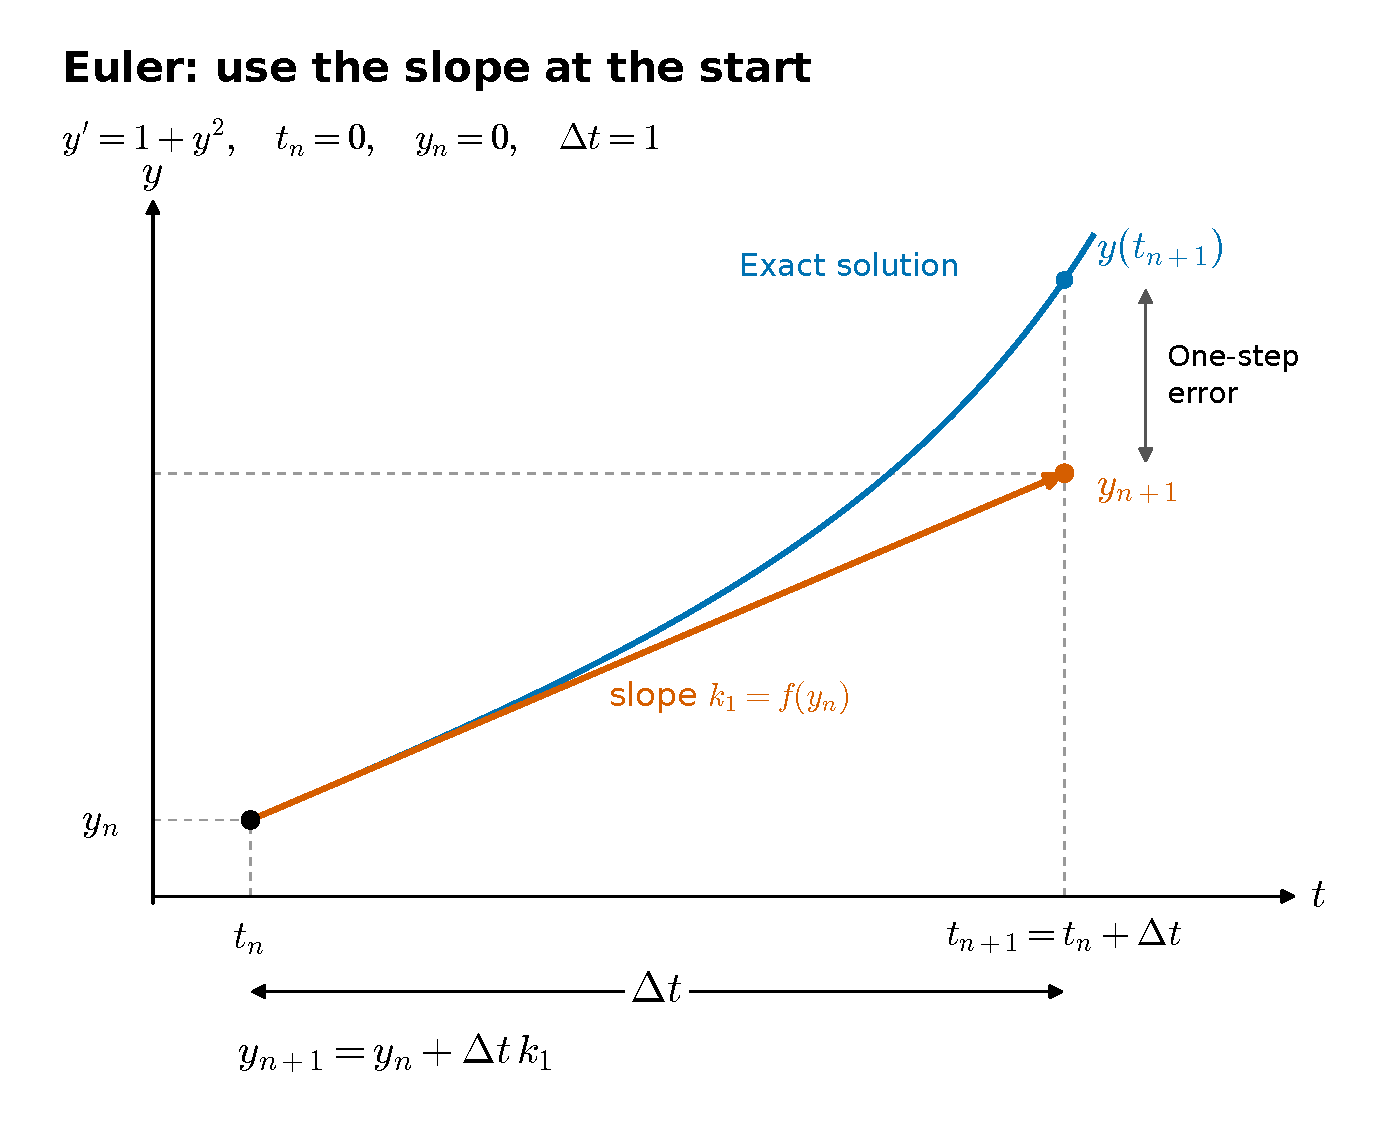
\includegraphics[width=0.60\linewidth]{ch03_euler_geometry.pdf}
\caption{Euler 法の1ステップ。青い曲線は厳密解 $y(t)=\tan t$、朱色の直線は始点の傾き $k_1=f(y_n)$ を用いた更新を表す。下の横矢印は時間幅 $\Delta t$、右の縦矢印は同じ終端時刻における厳密解と数値近似の差を示す。始点を厳密に与えているため、この差の大きさが1ステップの局所打ち切り誤差の大きさに対応する。}
\label{fig:ch3-euler-geometry}
\end{figure}

時刻 $t_n$ の値が厳密であるとして、1ステップで生じるずれを\textbf{局所打ち切り誤差}と呼ぶ。
Euler 法では、省略した最初の項から、この誤差は $O(\Delta t^2)$ である。
一方、更新を繰り返して得られる数値解には、それまでの局所的な誤差が伝播・累積した\textbf{大域誤差}が含まれる。
滑らかな右辺に対して十分小さい時間刻みを用い、固定した終端時刻まで積分すると、Euler 法の大域誤差は $O(\Delta t)$ となり、1次精度である\cite{kouya2021}。
この収束次数は §\ref{sec:ch3-convergence}で数値的に測定する。

式\eqref{eq:ch3-euler}を位置と速度へ書き戻すと、
\begin{align}
 \boldsymbol{x}_{n+1}&=\boldsymbol{x}_n+\Delta t\,\boldsymbol{v}_n,\label{eq:ch3-euler-x}\\
 \boldsymbol{v}_{n+1}&=\boldsymbol{v}_n+\Delta t\,\boldsymbol{g}(\boldsymbol{x}_n).\label{eq:ch3-euler-v}
\end{align}
これらの更新式を Python に対応させたものが Listing 3.1 である。
\begin{listingbox}{3.1　Euler 法の1ステップ}
\begin{Verbatim}[fontsize=\small]
# 位置と速度の両方を、更新前の値から求める
x_new = x + dt * v
v_new = v + dt * acc_func(x)
\end{Verbatim}
\end{listingbox}
ここで、\texttt{acc\_func} は、位置を受け取って加速度を返す関数を表す引数である。
Plummer 球の軌道計算では、前節で定義した\texttt{acc\_plummer\_model} を指定する。
このように加速度関数を指定することで、同じ時間積分法を異なる重力ポテンシャルにも適用できる。
また、\texttt{dt} は時間刻み $\Delta t$ を表す。

Euler 法では、位置と速度の両方を時刻 $t_n$ の値から計算する。
したがって、速度の更新に用いる加速度は、更新後の位置 \texttt{x\_new} ではなく、
更新前の位置 \texttt{x} から求める。
この1ステップの処理を時間ループで繰り返す実装は、§\ref{sec:ch3-circular-test}で示す。

% =====================================================================
\section{古典的4次 Runge--Kutta 法（RK4）}
\label{sec:ch3-rk4}

Euler 法は、1ステップの始点での変化率だけを使う。
Runge--Kutta 法では、時間区間内の状態を予測して右辺を複数回評価し、その結果を組み合わせて高い精度を得る。
古典的4次 Runge--Kutta 法（RK4）では、次の4つの変化率を計算する。
\begin{align}
 \boldsymbol{k}_1&=\boldsymbol{f}(\boldsymbol{y}_n),\label{eq:ch3-rk-k1}\\
 \boldsymbol{k}_2&=\boldsymbol{f}\left(\boldsymbol{y}_n+\frac{\Delta t}{2}\boldsymbol{k}_1\right),\label{eq:ch3-rk-k2}\\
 \boldsymbol{k}_3&=\boldsymbol{f}\left(\boldsymbol{y}_n+\frac{\Delta t}{2}\boldsymbol{k}_2\right),\label{eq:ch3-rk-k3}\\
 \boldsymbol{k}_4&=\boldsymbol{f}\left(\boldsymbol{y}_n+\Delta t\,\boldsymbol{k}_3\right).\label{eq:ch3-rk-k4}
\end{align}
$\boldsymbol{k}_1$ は始点での変化率、$\boldsymbol{k}_2$ と $\boldsymbol{k}_3$ は中間時刻、$\boldsymbol{k}_4$ は終点時刻の予測状態での変化率である。
$\boldsymbol{k}_2$ と $\boldsymbol{k}_3$ は同じ中間時刻に対応するが、その評価に用いる状態の予測値が異なる。
これらを使って、
\begin{equation}
 \boxed{\boldsymbol{y}_{n+1}=\boldsymbol{y}_n+\frac{\Delta t}{6}
 \left(\boldsymbol{k}_1+2\boldsymbol{k}_2+2\boldsymbol{k}_3+\boldsymbol{k}_4\right)}
\label{eq:ch3-rk4}
\end{equation}
と更新する\cite{kouya2021}。

\subsection{RK4の幾何学的説明}
図\ref{fig:ch3-rk4-geometry}では、図\ref{fig:ch3-euler-geometry}と同じ $dy/dt=1+y^2$ の例を使い、4つの傾きと最終更新を一つの $t$--$y$ 平面に示す。
図中の $Y_2,Y_3,Y_4$ は、それぞれ $k_2,k_3,k_4$ を評価するための予測値であり、
\begin{equation*}
 Y_2=y_n+\frac{\Delta t}{2}k_1,\qquad
 Y_3=y_n+\frac{\Delta t}{2}k_2,\qquad
 Y_4=y_n+\Delta t\,k_3
\end{equation*}
と書ける。
いずれも元の $y_n$ を基準に作る値であり、$Y_2$ と $Y_3$ は同じ中間時刻 $t_n+\Delta t/2$ に対する異なる予測である。
これらは厳密解の曲線上にあるとは限らない。

4つの傾きがそろったら、重み付き平均 $\bar{k}=(k_1+2k_2+2k_3+k_4)/6$ を求め、始点から $y_{n+1}=y_n+\Delta t\,\bar{k}$ と更新する。
この例では、$Y_4\simeq1.3906$ に対して最終値は $y_{n+1}\simeq1.5358$ となり、厳密解 $y(1)\simeq1.5574$ に近い。
最後の予測値 $Y_4$ をそのまま採用するのではなく、4つの傾きを組み合わせて次の値を決める点が重要である。

\begin{figure}[!htbp]
\centering
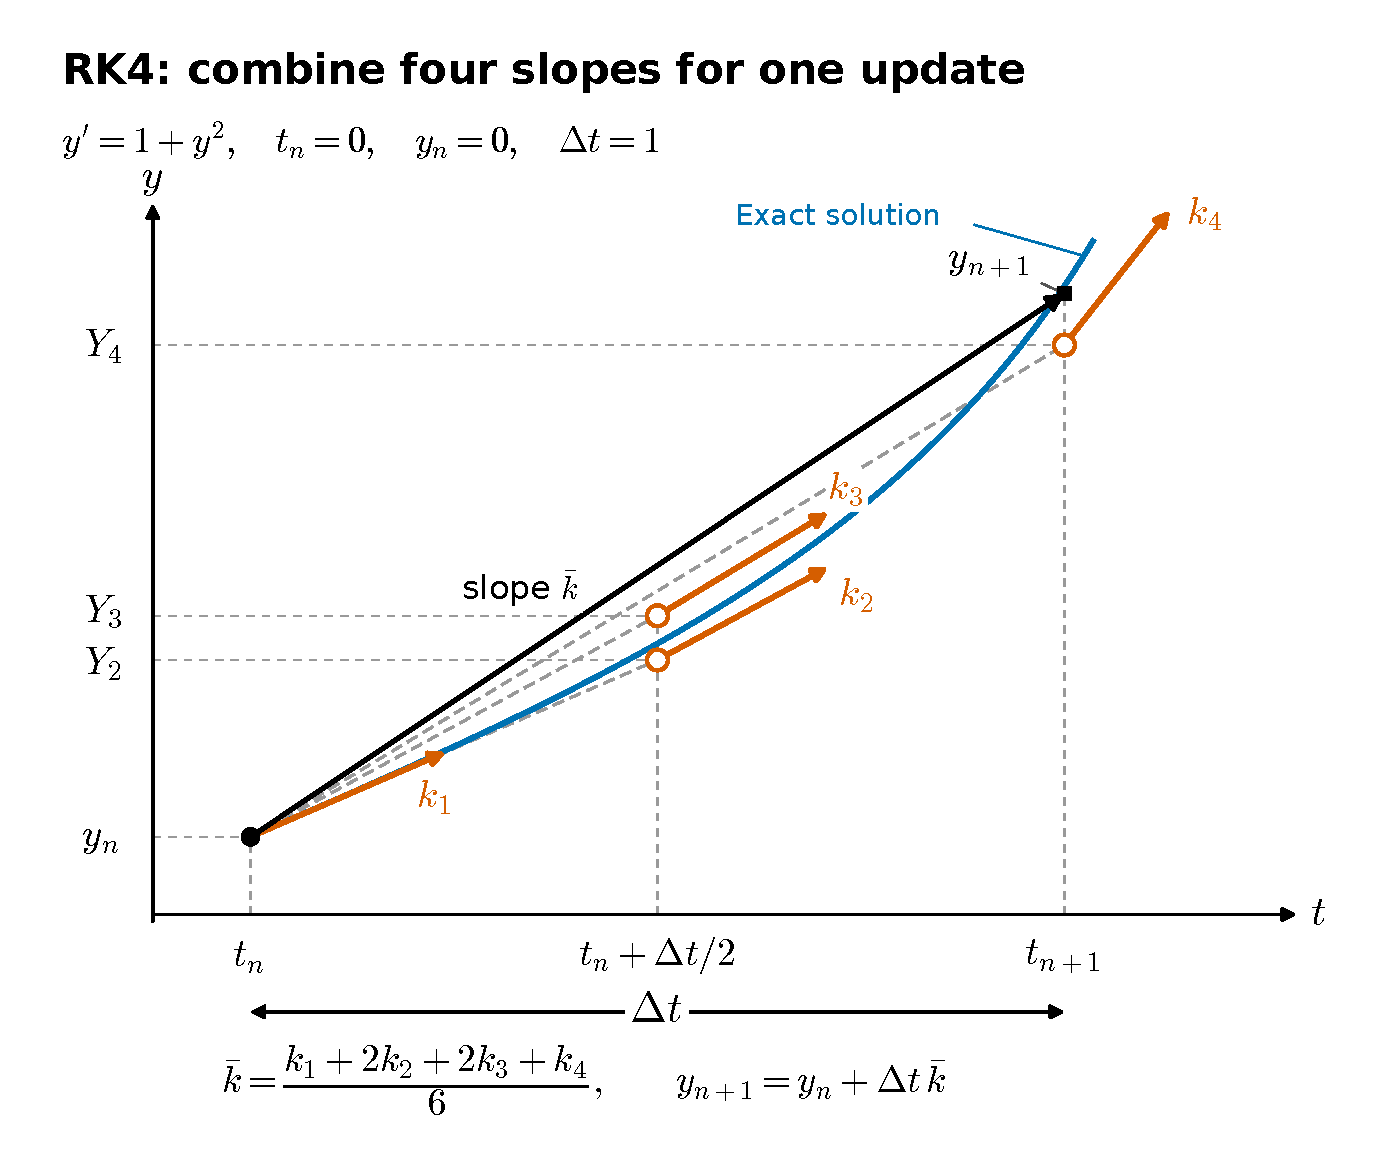
\includegraphics[width=0.60\linewidth]{ch03_rk4_geometry.pdf}
\caption{RK4 の4つの傾きと1ステップの更新。青い曲線は厳密解、白丸は予測値 $Y_2,Y_3,Y_4$、朱色の短い矢印は各評価点での傾き $k_1,k_2,k_3,k_4$ を表す。灰色の斜めの破線は始点から予測値を作る操作を示す。黒い矢印は平均傾き $\bar{k}$ を用いた最終更新であり、その終点の黒四角が $y_{n+1}$ である。この矢印や予測値を結ぶ線は、ステップ途中の解の曲線を表すものではない。}
\label{fig:ch3-rk4-geometry}
\end{figure}

中間状態の作り方と重み $1:2:2:1$ の組み合わせにより、厳密解の Taylor 展開と $\Delta t$ の4次まで一致する。
滑らかな右辺に対し、1ステップの局所打ち切り誤差は $O(\Delta t^5)$ である。
十分小さい時間刻みで固定した終端時刻まで積分したときの大域誤差は $O(\Delta t^4)$ となり、4次精度である。
ここでは更新式の使い方を学び、次数は円軌道の収束試験でも確かめる。

Notebook では、状態ベクトルを位置と速度の順に連結した1本の配列として扱う。
\texttt{ndim} は空間の次元数で、本章の平面内の運動では2である。
また、\texttt{y[n]} は時刻 $t_n$ の状態ベクトルを表す。

Listing 3.2 に、RK4 法の1ステップの計算を示す。
\begin{listingbox}{3.2　古典的4次 Runge--Kutta 法の1ステップ}
\begin{Verbatim}[fontsize=\small]
# 状態ベクトルから位置と速度を取り出し、時間微分を計算する
def rhs(state):
    x = state[:ndim]
    v = state[ndim:]
    return np.concatenate([v, acc_func(x)])

# 4つの予測状態で変化率を求め、次の状態を計算する
yn = y[n]
k1 = rhs(yn)
k2 = rhs(yn + 0.5 * dt * k1)
k3 = rhs(yn + 0.5 * dt * k2)
k4 = rhs(yn + dt * k3)
y[n + 1] = yn + dt * (k1 + 2*k2 + 2*k3 + k4) / 6.0
\end{Verbatim}
\end{listingbox}
ここで、\texttt{rhs} は式\eqref{eq:ch3-rhs}に対応し、状態ベクトルからその時間微分を計算する関数である。
\texttt{state[:ndim]} と \texttt{state[ndim:]} は、状態ベクトルから位置と速度をそれぞれ取り出す。
また、\texttt{np.concatenate} は複数の配列を一つにつなぐ関数であり、
ここでは速度と加速度をまとめて、状態ベクトルの時間微分を作る。

RK4 法は Euler 法より高次精度であるが、1ステップで右辺を4回評価する。
積分法を選ぶ際には、必要な精度だけでなく、計算コストも考慮する必要がある。
例えば、$N_{\rm p}$ 個の粒子間の重力を直接計算する重力多体系では、
全粒子対の重力を評価するため、1回の加速度計算に
$O(N_{\rm p}^2)$ の計算量がかかる\cite{tomisaka2007}。
このような計算では、時間積分法が必要とする加速度の評価回数も重要になる。

% =====================================================================
\section{リープフロッグ法（蛙跳び法）}
\label{sec:ch3-leapfrog}

本章のように加速度が位置だけで決まる場合には、
運動方程式を
\begin{equation}
 \ddot{\boldsymbol{x}}=\boldsymbol{g}(\boldsymbol{x})
\label{eq:ch3-second-order}
\end{equation}
と書ける。ドットは時間に関する微分を表す。
この式は、位置と速度に関する2つの一階微分方程式
\begin{align}
 \dot{\boldsymbol{x}}&=\boldsymbol{v},\\
 \dot{\boldsymbol{v}}&=\boldsymbol{g}(\boldsymbol{x})
\end{align}
に分けられる。

ここで、速度の変化率は位置だけで決まり、位置の変化率は速度だけで決まることに注目する。
この性質を利用すると、時間積分を2つの簡単な操作に分けて考えられる。
一つは、位置を固定して速度だけを更新する操作であり、キック（kick）と呼ぶ。
もう一つは、速度を固定して位置だけを更新する操作であり、ドリフト（drift）と呼ぶ。
リープフロッグ法は、この2つの操作を組み合わせて時間積分を行う方法である。

キックとドリフトを組み合わせる方法には、
キック--ドリフト--キック（kick--drift--kick; KDK）形式と、
ドリフト--キック--ドリフト（drift--kick--drift; DKD）形式がある。
どちらも2次精度のリープフロッグ法である。
本章ではKDK形式を用いる。この方法では、位置の更新（ドリフト）を
2つの半ステップの速度更新（キック）ではさむ。
この対称的な構成により、2次精度の時間積分法となる。

\subsection{KDKリープフロッグ法}
まず速度を半ステップ更新し、
\begin{equation}
 \boldsymbol{v}_{n+1/2}=\boldsymbol{v}_n+\frac{\Delta t}{2}\boldsymbol{g}(\boldsymbol{x}_n),
\label{eq:ch3-kick1}
\end{equation}
その補助速度で位置を1ステップ更新する。
\begin{equation}
 \boldsymbol{x}_{n+1}=\boldsymbol{x}_n+\Delta t\,\boldsymbol{v}_{n+1/2}.
\label{eq:ch3-drift}
\end{equation}
次に、新しい位置で加速度を評価し、速度を残り半ステップ更新する。
\begin{equation}
 \boldsymbol{v}_{n+1}=\boldsymbol{v}_{n+1/2}+\frac{\Delta t}{2}\boldsymbol{g}(\boldsymbol{x}_{n+1}).
\label{eq:ch3-kick2}
\end{equation}
すなわち、
\begin{equation}
 \boldsymbol{v}_n\rightarrow\boldsymbol{v}_{n+1/2}\rightarrow\boldsymbol{x}_{n+1}\rightarrow\boldsymbol{v}_{n+1}
\label{eq:ch3-leapfrog-flow}
\end{equation}
という計算順序で位置と速度を更新する。
ここで $\boldsymbol{v}_{n+1/2}$ は計算途中の補助速度であり、
この一連の操作で時刻 $t_n$ から $t_{n+1}=t_n+\Delta t$ まで進む。
一定の時間刻みでは、KDK形式で隣り合うステップの半ステップのキックをまとめると、
位置と速度を半ステップずれた時刻で交互に更新する形になる。
リープフロッグ（蛙跳び）という名前は、この互い違いの更新に由来する。
図\ref{fig:ch3-kdk}に、その時間的な配置を示す。
\begin{figure}[!htbp]
\centering
\begin{tikzpicture}[x=1.15cm,y=0.75cm,>=Latex,font=\sffamily\small]
% 時間軸：整数時刻に位置、半整数時刻に速度を配置
\draw[->,thick] (-0.5,0) -- (8.55,0) node[right] {$t$};
\foreach \i/\lab in {0/{n-2},2/{n-1},4/{n},6/{n+1},8/{n+2}}{
  \draw (\i,0.12) -- (\i,-0.12);
  \node[below=4pt] at (\i,-0.12) {$t_{\lab}$};
}
\foreach \i/\lab in {1/{n-\frac{3}{2}},3/{n-\frac{1}{2}},5/{n+\frac{1}{2}},7/{n+\frac{3}{2}}}{
  \draw[navy!85] (\i,0.12) -- (\i,-0.12);
  \node[above=4pt] at (\i,0.12) {$t_{\lab}$};
}
% 速度は位置の時刻を飛び越して更新する（Kick）
\foreach \i/\j in {1/3,3/5,5/7}{
  \draw[->,thick,navy!85] (\i,1.17)
    .. controls + (0.55,0.70) and +(-0.55,0.70) .. (\j,1.17);
}
% 位置は速度の時刻を飛び越して更新する（Drift）
\foreach \i/\j in {0/2,2/4,4/6,6/8}{
  \draw[->,thick,black!75] (\i,-1.17)
    .. controls + (0.55,-0.70) and +(-0.55,-0.70) .. (\j,-1.17);
}
\node[text=navy!85] at (4,2.05) {Velocity (Kick)};
\node[text=black!75] at (4,-2.05) {Position (Drift)};
\end{tikzpicture}
\caption{リープフロッグ法における位置と速度の時間的な配置。
位置は整数時刻、速度は半整数時刻に対応する。
上側の矢印は速度の更新（kick）、下側の矢印は位置の更新（drift）を表す。
位置と速度が半ステップずれて交互に更新されることが、「蛙跳び」という名前の由来である。}
\label{fig:ch3-kdk}
\end{figure}

式\eqref{eq:ch3-kick1}--\eqref{eq:ch3-kick2}は、Listing 3.3 の3行に対応する。

\begin{listingbox}{3.3　リープフロッグ法の1ステップ}
\begin{Verbatim}[fontsize=\small]
# 速度を半ステップ、位置を1ステップ、速度を半ステップ更新する
v_half = v + 0.5 * dt * acc_func(x)
x_new = x + dt * v_half
v_new = v_half + 0.5 * dt * acc_func(x_new)
\end{Verbatim}
\end{listingbox}

リープフロッグ法は、滑らかな加速度に対して2次精度の時間積分法である。
その収束次数は §\ref{sec:ch3-convergence}の数値実験で確認する。
更新式から誤差次数を求める計算は、以下の補足に示す。

Listing 3.3 では、各ステップの最初と最後に加速度を計算している。
しかし、前のステップの最後に求めた加速度は、
次のステップの最初にも使えるため、保存して再利用すれば計算回数を減らせる。
本書では、更新式との対応を分かりやすくするため、加速度を毎回計算している。

\begin{topicblock}{リープフロッグ法が2次精度になる理由}
時刻 $t_n$ の位置と速度が厳密であるとして、1ステップの誤差を調べる。
最初の速度更新を位置更新へ代入すると、
\begin{equation}
 \boldsymbol{x}_{n+1}=\boldsymbol{x}_n+\Delta t\,\boldsymbol{v}_n+\frac{\Delta t^2}{2}\boldsymbol{g}(\boldsymbol{x}_n)
\label{eq:ch3-leapfrog-position-combined}
\end{equation}
となる。これは位置の Taylor 展開を2次まで残した式である。
滑らかな加速度なら、厳密解の次項は $\Delta t^3\dot{\boldsymbol{g}}_n/6$ である。
ここで $\dot{\boldsymbol{g}}_n$ は、軌道に沿った加速度の時間微分を $t_n$ で評価した値を表す。
したがって、位置の局所打ち切り誤差は $O(\Delta t^3)$ である。

2回の速度更新をまとめると、
\begin{equation}
 \boldsymbol{v}_{n+1}=\boldsymbol{v}_n+\frac{\Delta t}{2}
 \left[\boldsymbol{g}(\boldsymbol{x}_n)+\boldsymbol{g}(\boldsymbol{x}_{n+1})\right]
\label{eq:ch3-leapfrog-velocity-combined}
\end{equation}
となる。一方、厳密な速度変化は
\begin{equation}
 \boldsymbol{v}(t_{n+1})-\boldsymbol{v}(t_n)=\int_{t_n}^{t_{n+1}}\boldsymbol{g}(\boldsymbol{x}(t))\,dt
\end{equation}
である。
式\eqref{eq:ch3-leapfrog-velocity-combined}は、加速度の時間積分に第1章の台形則を適用した形になっている。
厳密な端点加速度を用いた場合、台形則による1区間の誤差は $O(\Delta t^3)$ である。

実際には、終点の加速度を数値的な位置 $\boldsymbol{x}_{n+1}$ で評価する。
この位置には $O(\Delta t^3)$ の誤差があるため、滑らかな加速度では、その評価値の誤差も $O(\Delta t^3)$ となる。
ただし、速度更新ではこれに $\Delta t/2$ を掛けるので、速度への寄与は $O(\Delta t^4)$ である。
この寄与は台形則の主要な誤差より高次であり、速度の局所打ち切り誤差は $O(\Delta t^3)$ のままである。

固定した終端時刻までのステップ数は $O(\Delta t^{-1})$ である。
滑らかな力に対して安定に積分できる範囲では、局所的な誤差の伝播・累積を含めた位置と速度の大域誤差は、ともに $O(\Delta t^2)$ となる。
これがリープフロッグ法の2次精度に対応する。
\end{topicblock}
% =====================================================================
\section{円軌道による時間積分法の検証}
\label{sec:ch3-circular-test}

ここまでに示した3つの更新式を繰り返して、実際に軌道を計算する。
まず位置の解析解が分かる円軌道を用い、同じ初期条件と時間刻みで得た結果を比較する。

\subsection{円軌道の解析解}

半径 $r_0$ の円軌道の角速度を $\Omega$ とする。
円運動に必要な向心加速度の大きさと重力加速度の大きさを等しくすると、
\begin{equation}
 \Omega^2r_0=\frac{GMr_0}{(r_0^2+a^2)^{3/2}}
\end{equation}
であるから、
\begin{equation}
 \Omega^2=\frac{GM}{(r_0^2+a^2)^{3/2}}
\label{eq:ch3-plummer-omega}
\end{equation}
を得る。円運動速度と周期は、それぞれ
\begin{equation}
 v_{\rm circ}=\Omega r_0,\qquad T_0=\frac{2\pi}{\Omega}
\label{eq:ch3-plummer-period}
\end{equation}
である。
Notebook 3 と同じく $G=M=a=r_0=1$ とすると、
\begin{equation}
 \Omega=\chthreeOmegaPlummer,\qquad
 v_{\rm circ}=\chthreeVcPlummer,\qquad
 T_0=\chthreePeriodPlummer
\label{eq:ch3-plummer-numbers}
\end{equation}
となる。角速度の単位は $t_\ast^{-1}$ で、速度と周期の単位は式\eqref{eq:ch3-dynamical-units}に示したものである。

初期条件
\begin{equation}
 (x,y)=(r_0,0),\qquad (v_x,v_y)=(0,v_{\rm circ})
\end{equation}
に対する解析的な位置は
\begin{equation}
 x(t)=r_0\cos\Omega t,\qquad y(t)=r_0\sin\Omega t
\label{eq:ch3-circular-exact}
\end{equation}
であり、数値軌道を検証する基準になる。

\subsection{時間ループと積分関数}

軌道全体を求めるには、初期位置と初期速度を配列に保存し、1ステップの更新を繰り返す。
この処理を、Euler 法、RK4、リープフロッグ法について、それぞれ \texttt{integrate\_euler}、\texttt{integrate\_rk4}、\texttt{integrate\_leapfrog} という関数にまとめる。
各関数には、加速度を返す関数 \texttt{acc\_func}、初期位置 \texttt{x0}、初期速度 \texttt{v0}、正の時間刻み \texttt{dt}、ステップ数 \texttt{nstep} を渡す。
初期位置と初期速度は、同じ次元数の1次元配列とする。

\texttt{nstep} 回更新すると、初期時刻を含めて \texttt{nstep + 1} 個の時刻の値が得られる。
返り値の \texttt{x} と \texttt{v} は、行が時刻、列が座標成分を表す配列である。
したがって、\texttt{x[n]} は時刻 $t_n$ の位置ベクトル、\texttt{x[-1]} は最終時刻の位置ベクトルに対応する。
\begin{notebookblock}{3｜時間ループと積分関数}
配列の準備、初期値の保存、時間ループ、結果の返却という構造は3つの関数に共通する。
時間ループ内の更新式が、Listing 3.1--3.3 に対応する。

\par\smallskip\noindent\begin{minipage}{\linewidth}
{\sffamily\small\color{graytext}対応セル（Euler 法）}
\begin{Verbatim}[xleftmargin=2mm,fontsize=\small,frame=single,framesep=1.8mm,framerule=0.35pt,rulecolor=\color{listingframe},fillcolor=\color{listingbg}]
def integrate_euler(acc_func, x0, v0, dt, nstep):
    # 小数を保持できる初期値と、全時刻の保存用配列を用意する
    x0 = np.asarray(x0, dtype=float)
    v0 = np.asarray(v0, dtype=float)
    ndim = len(x0)
    x = np.empty((nstep + 1, ndim))
    v = np.empty((nstep + 1, ndim))
    x[0], v[0] = x0, v0

    # 各ステップで、更新前の位置と速度から次の値を求める
    for n in range(nstep):
        x[n + 1] = x[n] + dt * v[n]
        v[n + 1] = v[n] + dt * acc_func(x[n])

    return x, v
\end{Verbatim}
\end{minipage}

\par\smallskip\noindent\begin{minipage}{\linewidth}
{\sffamily\small\color{graytext}対応セル（RK4）}
\begin{Verbatim}[xleftmargin=2mm,fontsize=\small,frame=single,framesep=1.8mm,framerule=0.35pt,rulecolor=\color{listingframe},fillcolor=\color{listingbg}]
def integrate_rk4(acc_func, x0, v0, dt, nstep):
    x0 = np.asarray(x0, dtype=float)
    v0 = np.asarray(v0, dtype=float)
    ndim = len(x0)
    y = np.empty((nstep + 1, 2 * ndim))
    y[0] = np.concatenate([x0, v0])

    # 状態の前半を位置、後半を速度として変化率を返す
    def rhs(state):
        x = state[:ndim]
        v = state[ndim:]
        return np.concatenate([v, acc_func(x)])

    # Listing 3.2 の更新を繰り返す
    for n in range(nstep):
        yn = y[n]
        k1 = rhs(yn)
        k2 = rhs(yn + 0.5 * dt * k1)
        k3 = rhs(yn + 0.5 * dt * k2)
        k4 = rhs(yn + dt * k3)
        y[n + 1] = yn + dt * (k1 + 2*k2 + 2*k3 + k4) / 6.0

    # 状態の履歴を、位置と速度の配列に分けて返す
    return y[:, :ndim], y[:, ndim:]
\end{Verbatim}
\end{minipage}

\par\smallskip\noindent\begin{minipage}{\linewidth}
{\sffamily\small\color{graytext}対応セル（リープフロッグ法）}
\begin{Verbatim}[xleftmargin=2mm,fontsize=\small,frame=single,framesep=1.8mm,framerule=0.35pt,rulecolor=\color{listingframe},fillcolor=\color{listingbg}]
def integrate_leapfrog(acc_func, x0, v0, dt, nstep):
    x0 = np.asarray(x0, dtype=float)
    v0 = np.asarray(v0, dtype=float)
    ndim = len(x0)
    x = np.empty((nstep + 1, ndim))
    v = np.empty((nstep + 1, ndim))
    x[0], v[0] = x0, v0

    # キック、ドリフト、キックの順に更新する
    for n in range(nstep):
        v_half = v[n] + 0.5 * dt * acc_func(x[n])
        x[n + 1] = x[n] + dt * v_half
        v[n + 1] = v_half + 0.5 * dt * acc_func(x[n + 1])

    return x, v
\end{Verbatim}
\end{minipage}
\end{notebookblock}

\subsection{1周期の軌道を比較する}

これらの関数を使い、円軌道の1周期 $T_0$ を $N=100$ ステップに分けて計算する。
コード中の \texttt{nstep} がステップ数 $N$ に対応し、時間刻みは $\Delta t=T_0/100$ である。
\begin{notebookblock}{3｜円軌道による時間積分法の比較}
初期条件と周期を準備し、3つの積分関数に同じ加速度・初期条件・時間刻みを渡す。
返された位置配列を使って、図\ref{fig:ch3-circular}を描く。

\par\smallskip\noindent\begin{minipage}{\linewidth}
{\sffamily\small\color{graytext}対応セル（初期条件と計算）}
\begin{Verbatim}[xleftmargin=2mm,fontsize=\small,frame=single,framesep=1.8mm,framerule=0.35pt,rulecolor=\color{listingframe},fillcolor=\color{listingbg}]
# 円軌道の角速度、円運動速度、周期を求める
r0 = 1.0
Omega0 = np.sqrt(G * M / (r0**2 + a**2)**1.5)
vc0 = Omega0 * r0
T0 = 2.0 * np.pi / Omega0
x0 = np.array([r0, 0.0])
v0 = np.array([0.0, vc0])

# 1周期を100ステップで積分する
nstep = 100
dt = T0 / nstep
x_eu, v_eu = integrate_euler(acc_plummer_model, x0, v0, dt, nstep)
x_lf, v_lf = integrate_leapfrog(acc_plummer_model, x0, v0, dt, nstep)
x_rk, v_rk = integrate_rk4(acc_plummer_model, x0, v0, dt, nstep)
\end{Verbatim}
\end{minipage}
\end{notebookblock}

\begin{figure}[!htbp]
\centering
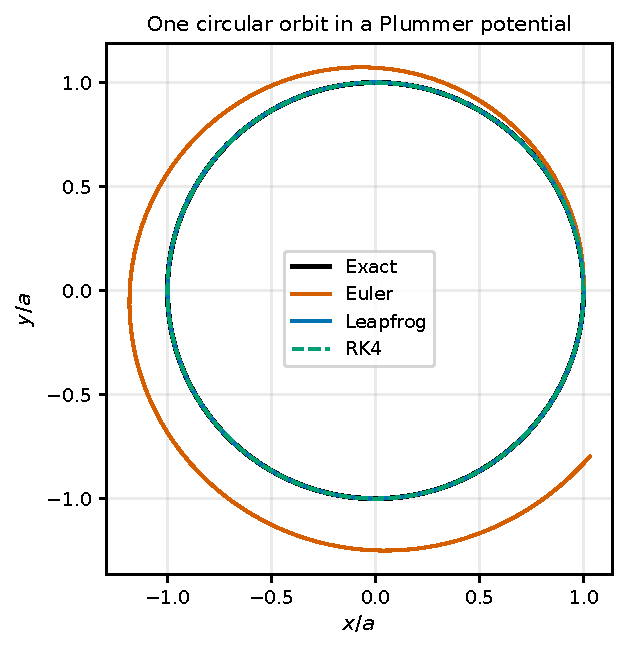
\includegraphics[width=0.62\linewidth]{ch03_circular_orbit.pdf}
\caption{1周期 $T_0$ を $N=100$ ステップで積分した円軌道。時間刻みは $\Delta t=T_0/100$ である。解析解と3つの時間積分法を比較している。}
\label{fig:ch3-circular}
\end{figure}

図\ref{fig:ch3-circular}では、Euler 法の軌道が外側へずれる一方、リープフロッグ法と RK4 は解析的な円軌道に近く見える。
ただし、一つの時間刻みで描いた軌道だけでは、誤差の大きさや収束次数を十分には判断できない。
次節では、解析解からの位置のずれを直接測り、時間刻みを変えたときの誤差の減少を調べる。
% =====================================================================
\section{時間積分法の収束次数}
\label{sec:ch3-convergence}

前節では、一つの時間刻みで1周期の軌道を描いた。
本節では終端時刻を固定し、時間刻みを変えて同じ計算を繰り返す。
第\ref{sec:ch1-convergence}節の格子収束試験で格子幅を変えたのと同じ考え方で、時間積分法の収束次数を測定する。

ここでは、円軌道を90度進んだ時刻 $T_0/4$ を終端時刻とする。この時刻の厳密な位置は
\begin{equation}
 \boldsymbol{x}_{\rm exact}(T_0/4)=(0,r_0)
\end{equation}
と分かっているので、数値的な位置とのずれ
\begin{equation}
 \epsilon_x=\left|\boldsymbol{x}_{\rm num}(T_0/4)-\boldsymbol{x}_{\rm exact}(T_0/4)\right|
\label{eq:ch3-position-error}
\end{equation}
を直接測定できる。
縦棒はベクトルの大きさを表し、$\epsilon_x$ は二つの位置の間の距離である。
コードでは \texttt{np.linalg.norm} で計算する。

Notebook 3 では、$T_0/4$ までを $N=20,40,80,160,320$ ステップで積分する。
前節の1周期の計算とは異なり、ここでの時間刻みは $\Delta t=T_0/(4N)$ である。
誤差が $\epsilon_x\simeq C(\Delta t)^p$ に従う範囲では、両対数プロットの傾きが収束次数 $p$ となる。
$C$ は、終端時刻と初期条件を固定したときに時間刻みに依存しない係数である。
\begin{notebookblock}{3｜時間積分法の収束次数}
積分関数を辞書 \texttt{methods} にまとめ、手法と時間刻みを変えて計算する。
\texttt{errors} に位置誤差を保存し、5種類の時間刻みすべてを用いて両対数上で直線近似する。

\par\smallskip\noindent\begin{minipage}{\linewidth}
{\sffamily\small\color{graytext}対応セル（誤差と収束次数の測定）}
\begin{Verbatim}[xleftmargin=2mm,fontsize=\small,frame=single,framesep=1.8mm,framerule=0.35pt,rulecolor=\color{listingframe},fillcolor=\color{listingbg}]
# 3つの積分関数を、名前と対応させて登録する
methods = {
    "Euler": integrate_euler,
    "Leapfrog": integrate_leapfrog,
    "RK4": integrate_rk4,
}

# 終端時刻を固定し、試すステップ数と解析的な位置を用意する
N_values = np.array([20, 40, 80, 160, 320])
t_end = T0 / 4.0
x_exact_end = np.array([0.0, r0])
dt_values = t_end / N_values
errors = {}

# 最終時刻の位置のずれを距離として測る
for name, method in methods.items():
    err = []
    for N_i in N_values:
        dt_i = t_end / N_i
        x_i, v_i = method(acc_plummer_model, x0, v0, dt_i, int(N_i))
        err.append(np.linalg.norm(x_i[-1] - x_exact_end))
    errors[name] = np.array(err)

# 両対数上での直線の傾きを求める
orders = {}
for name, err in errors.items():
    orders[name] = np.polyfit(np.log(dt_values), np.log(err), 1)[0]
\end{Verbatim}
\end{minipage}
\end{notebookblock}

この計算から、
\begin{equation}
 p_{\rm Euler}=\chthreeOrderEuler,\qquad
 p_{\rm leapfrog}=\chthreeOrderLeapfrog,\qquad
 p_{\rm RK4}=\chthreeOrderRKFour
\label{eq:ch3-orders}
\end{equation}
を得る。
Euler 法はほぼ1次、リープフロッグ法はほぼ2次、RK4 はほぼ4次精度で収束している。
時間刻みを半分にすると、誤差はそれぞれおよそ $1/2$、$1/4$、$1/16$ に減少する。
図\ref{fig:ch3-convergence}の点列の傾きは、この誤差の減少を表している。

\begin{figure}[!htbp]
\centering
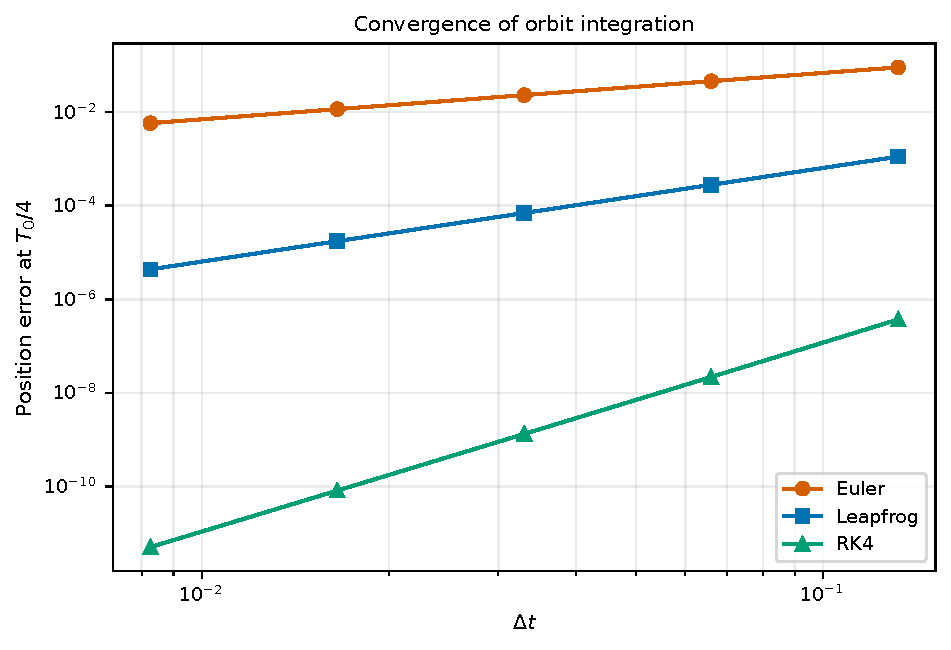
\includegraphics[width=0.66\linewidth]{ch03_convergence.pdf}
\caption{円軌道の $T_0/4$ 後の位置誤差と時間刻みの関係。両対数表示の傾きから、Euler 法・リープフロッグ法・RK4 の大域収束次数を測定する。}
\label{fig:ch3-convergence}
\end{figure}
% =====================================================================
\section{保存量による数値軌道の診断}
\label{sec:ch3-invariants}

前節では、円軌道の解析解と比較して位置の誤差を測った。
軌道計算では、このような直接比較に加えて、本来一定である保存量が数値計算でも保たれているかを調べることができる。
本節では、半径が時間とともに変化する離心軌道を用い、エネルギーと角運動量から数値軌道を診断する。

単位質量あたりのエネルギーを\textbf{比エネルギー（specific energy）}と呼び、
\begin{equation}
 E=\frac12v^2+\Phi(r)
\label{eq:ch3-energy}
\end{equation}
と定義する。ここで $v=|\boldsymbol{v}|$ である。
また、単位質量あたりの角運動量を\textbf{比角運動量（specific angular momentum）}と呼び、
\begin{equation}
 \boldsymbol{L}=\boldsymbol{x}\times\boldsymbol{v}
\label{eq:ch3-angular-momentum}
\end{equation}
と定義する。
以下では、これらを単にエネルギー、角運動量と呼ぶ。
ポテンシャルが時間に依存しないためエネルギーが保存され、球対称な重力場の力が中心方向を向くため角運動量が保存される。
したがって、厳密な運動では
\begin{equation}
 \boxed{E=\mathrm{const.},\qquad\boldsymbol{L}=\mathrm{const.}}
\label{eq:ch3-spherical-invariants}
\end{equation}
である\cite{ryden2025}。
本章の $x$--$y$ 平面内の運動では、その平面に垂直な成分 $L_z=xv_y-yv_x$ を診断に用いる。

Notebook 3 では、$G=M=a=1$ の単位で
\begin{equation}
 \boldsymbol{x}_0=(1,0),\qquad\boldsymbol{v}_0=(0,0.45)
\label{eq:ch3-eccentric-ic}
\end{equation}
とする。
初速度をこの半径の円運動速度より小さくすることで、半径が変化する軌道を作る。
$\Delta t=T_0/100$ で、基準周期の20倍の時間 $20T_0$ まで2000ステップで積分する。
$T_0$ は式\eqref{eq:ch3-plummer-period}の円軌道の基準周期であり、この離心軌道の実測周期ではない。

計算した各時刻で保存量を評価し、初期値からの相対的なずれ
\begin{equation}
 \frac{E(t)-E(0)}{|E(0)|},\qquad
 \frac{L_z(t)-L_z(0)}{|L_z(0)|}
\label{eq:ch3-relative-invariants}
\end{equation}
を求める。今回の初期条件では、どちらの分母も0ではない。
これらの量が0からどれだけずれるかを調べることで、保存量が数値計算でどの程度保たれているかを確認できる。
\begin{notebookblock}{3｜離心軌道と保存量}
前節で定義した \texttt{methods} を使い、同じ初期条件を3つの方法で積分する。
\texttt{orbits} に軌道と保存量を保存し、\texttt{relative\_errors} に式\eqref{eq:ch3-relative-invariants}の符号付きのずれを保存する。

\par\smallskip\noindent\begin{minipage}{\linewidth}
{\sffamily\small\color{graytext}対応セル（保存量を計算する関数）}
\begin{Verbatim}[xleftmargin=2mm,fontsize=\small,frame=single,framesep=1.8mm,framerule=0.35pt,rulecolor=\color{listingframe},fillcolor=\color{listingbg}]
# 全時刻の位置・速度配列から、各時刻の比エネルギーを返す
def energy_plummer(x, v, G, M, a):
    return 0.5 * np.sum(v**2, axis=1) + phi_plummer_pos(x, G, M, a)

# 平面内の運動に対する比角運動量の z 成分を返す
def angular_momentum_z(x, v):
    return x[:, 0] * v[:, 1] - x[:, 1] * v[:, 0]
\end{Verbatim}
\end{minipage}

\par\smallskip\noindent\begin{minipage}{\linewidth}
{\sffamily\small\color{graytext}対応セル（軌道と保存量の計算）}
\begin{Verbatim}[xleftmargin=2mm,fontsize=\small,frame=single,framesep=1.8mm,framerule=0.35pt,rulecolor=\color{listingframe},fillcolor=\color{listingbg}]
# 離心軌道の初期条件と計算時間を設定する
x0_e = np.array([1.0, 0.0])
v0_e = np.array([0.0, 0.45])
n_period = 20
steps_per_period = 100
dt = T0 / steps_per_period
nstep = n_period * steps_per_period
t = np.arange(nstep + 1) * dt

# 各手法の軌道と保存量の履歴を保存する
orbits = {}
for name, method in methods.items():
    x_i, v_i = method(acc_plummer_model, x0_e, v0_e, dt, nstep)
    E_i = energy_plummer(x_i, v_i, G, M, a)
    L_i = angular_momentum_z(x_i, v_i)
    orbits[name] = (x_i, v_i, E_i, L_i)
\end{Verbatim}
\end{minipage}

\par\smallskip\noindent\begin{minipage}{\linewidth}
{\sffamily\small\color{graytext}対応セル（保存量の相対変化）}
\begin{Verbatim}[xleftmargin=2mm,fontsize=\small,frame=single,framesep=1.8mm,framerule=0.35pt,rulecolor=\color{listingframe},fillcolor=\color{listingbg}]
# 符号付きの相対変化と、その絶対値の最大値を求める
relative_errors = {}
short_max_errors = {}
for name in methods:
    E_i, L_i = orbits[name][2:]
    relE = (E_i - E_i[0]) / abs(E_i[0])
    relL = (L_i - L_i[0]) / abs(L_i[0])
    relative_errors[name] = (relE, relL)
    max_E = np.max(np.abs(relE))
    max_L = np.max(np.abs(relL))
    short_max_errors[name] = {"energy": max_E, "Lz": max_L}
\end{Verbatim}
\end{minipage}
\end{notebookblock}

図\ref{fig:ch3-eccentric}に計算した軌道を示す。
Euler 法では軌道が外側へ広がる一方、リープフロッグ法と RK4 は中心付近の限られた範囲を運動する。
この違いを、保存量の変化から調べる。

\begin{figure}[!htbp]
\centering
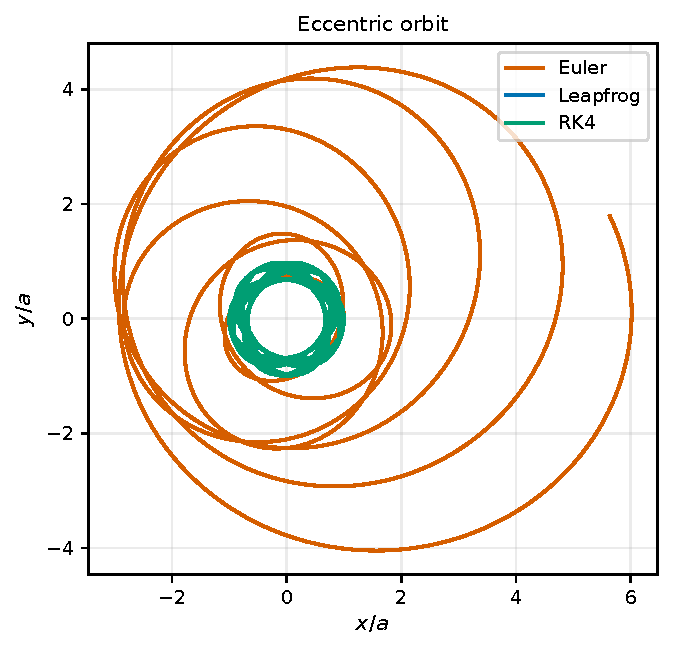
\includegraphics[width=0.52\linewidth]{ch03_eccentric_orbit.pdf}
\caption{Plummer ポテンシャル中の離心軌道。初期条件は式\eqref{eq:ch3-eccentric-ic}で、3手法を同じ $\Delta t=T_0/100$ により $20T_0$ まで積分している。}
\label{fig:ch3-eccentric}
\end{figure}

図\ref{fig:ch3-energy-error}では、式\eqref{eq:ch3-relative-invariants}のエネルギーのずれの絶対値を、対数目盛で比較している。
この時間刻みと積分時間では、最大絶対相対変化はリープフロッグ法で $\chthreeShortMaxEnergyLeapfrog$、RK4 で $\chthreeShortMaxEnergyRKFour$ となり、RK4 の方が小さい。
Euler 法の誤差はこれらより大きく、外側へ広がる軌道に対応してエネルギーも変化している。

\begin{figure}[!htbp]
\centering
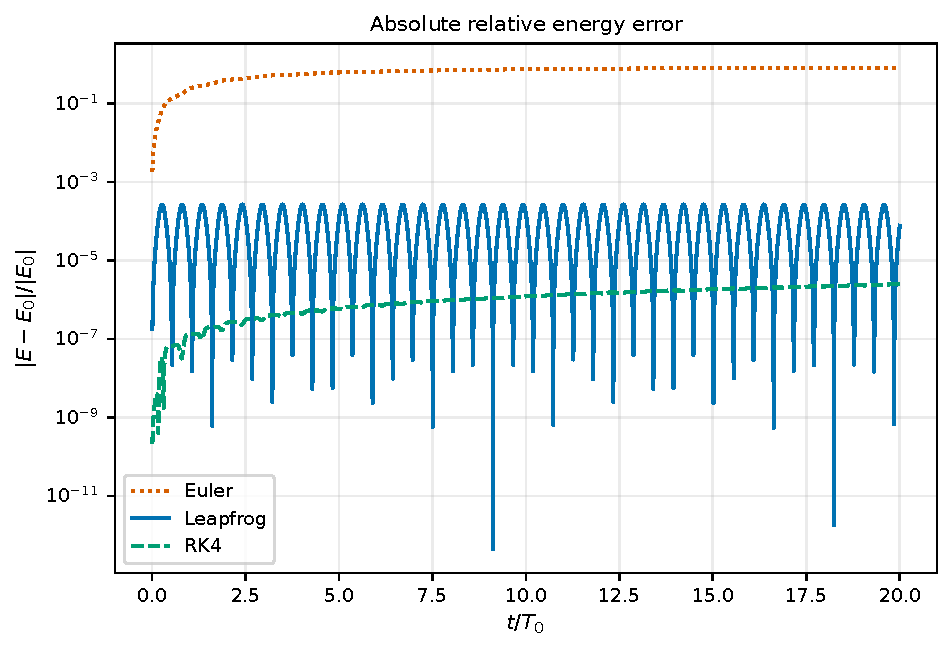
\includegraphics[width=0.65\linewidth]{ch03_energy_error.pdf}
\caption{離心軌道における $|E(t)-E(0)|/|E(0)|$。条件は $\Delta t=T_0/100$、積分時間 $20T_0$ である。縦軸は対数目盛で、誤差が0の点は表示していない。リープフロッグ法の下向きの鋭い谷は、符号付き誤差が0に近づいて絶対値が一時的に小さくなる時刻に対応し、その瞬間に軌道全体が高精度になったことを意味しない。}
\label{fig:ch3-energy-error}
\end{figure}

角運動量のずれを図\ref{fig:ch3-lz-error}に示す。
リープフロッグ法では、角運動量のずれは非常に小さい。
中心力の場合、キックで加える速度変化は位置ベクトルに平行であり、ドリフトで加える位置変化はその段階の速度に平行である。
このため、それぞれの更新で $\boldsymbol{x}\times\boldsymbol{v}$ は変わらず、角運動量は浮動小数点演算による誤差を除いて保存される。

\begin{figure}[!htbp]
\centering
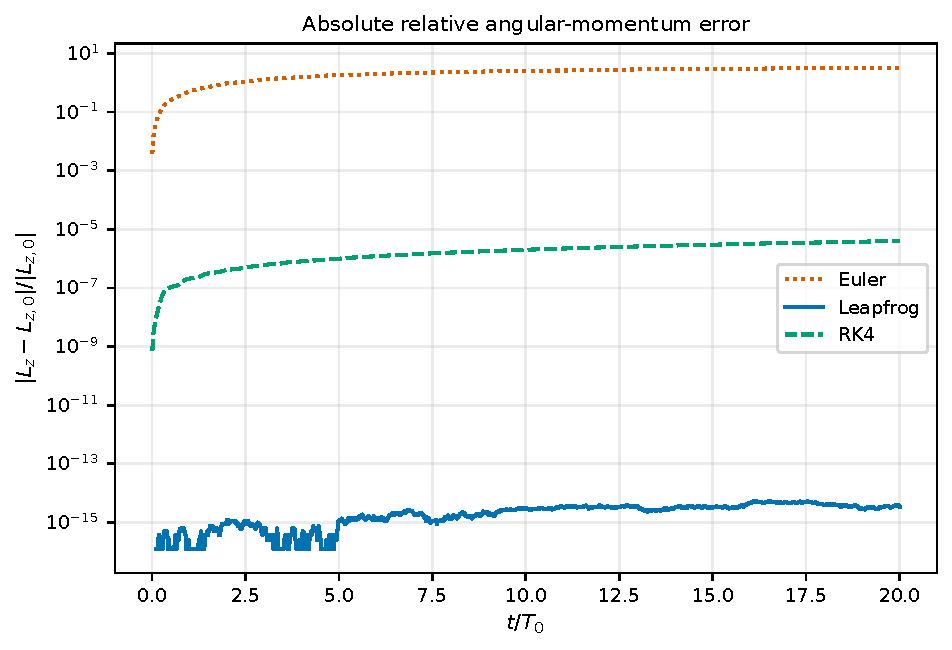
\includegraphics[width=0.65\linewidth]{ch03_angular_momentum_error.pdf}
\caption{同じ計算における $|L_z(t)-L_z(0)|/|L_z(0)|$。縦軸は対数目盛で、誤差が0の点は表示していない。
リープフロッグ法では角運動量が理論上厳密に保存されるが、実際の計算では浮動小数点演算によるわずかなずれが生じる。}
\label{fig:ch3-lz-error}
\end{figure}

ただし、角運動量が保存されていても、数値軌道が正確とは限らない。
例えば、円軌道では角運動量が一定でも、軌道位相に誤差が生じると、同じ時刻における恒星の位置は解析解からずれてしまう。
そのため、角運動量の保存だけでなく、解析解との比較や時間刻みを変えた収束試験によっても、
数値計算の精度を確かめる必要がある。

また、エネルギー誤差の大きさだけでなく、符号付きの時間変化にも違いがある。
リープフロッグ法では誤差が振動するのに対し、RK4 では一方向へのずれが見られる。
この符号付き誤差の拡大図は Notebook 3 で確認できる。
次節では、積分時間を長くして両者の違いを調べる。
% =====================================================================
保存量の選択は、解く問題によって変わる。
自己重力の $N$ 体計算では粒子間でエネルギーを交換するため、各粒子のエネルギーは一般には一定でない。
外力がなく、粒子質量が一定の孤立系では、系全体のエネルギーなどを保存量の診断に用いる\cite{tomisaka2007}。
本章で各軌道のエネルギーを調べるのは、粒子が動いても変わらない、時間に依存しない重力場を与えているためである。

\section{高次精度と長時間保存性の違い}
\label{sec:ch3-long-term}

前節の条件では、RK4 のエネルギー誤差はリープフロッグ法より小さかった。
しかし、その大小だけでは、さらに長い時間まで積分したときの誤差を判断できない。
本節では同じ離心軌道を長時間積分し、誤差が振動する場合と一方向にずれる場合の違いを比較する。

Notebook 3 では、$\Delta t=T_0/50$ で $1000T_0$ まで積分する。
$T_0$ は円軌道の基準周期である。
前節より積分時間が長いだけでなく、時間刻みも2倍なので、時間経過だけの影響を調べる際は、この長時間計算の最初の $20T_0$ と全体の $1000T_0$ を比べる。
手法間の比較は同じ時間刻みでの比較であり、同じ計算コストでの比較ではない。

符号付きのエネルギー誤差が振動する場合、最終値は計算を終えるタイミングによって変わる。
そこで、時間変化に加えて、終端時刻 $T$ までの出力時刻 $t_n$ で測った最大絶対相対変化
\begin{equation}
 \epsilon_{E,\max}(T)\equiv\max_{0\le t_n\le T}\frac{|E(t_n)-E(0)|}{|E(0)|}
\label{eq:ch3-max-energy-error}
\end{equation}
を用い、計算中に誤差がどこまで大きくなったかを比較する。
\begin{notebookblock}{3｜RK4 とリープフロッグ法の長時間挙動}
前節で定義した \texttt{x0\_e}、\texttt{v0\_e} を初期条件に用い、RK4 とリープフロッグ法で計算する。
\texttt{long\_results} には全時刻の符号付き誤差を、\texttt{long\_max\_errors} には二つの時間範囲の最大誤差を保存する。

\par\smallskip\noindent\begin{minipage}{\linewidth}
{\sffamily\small\color{graytext}対応セル（長時間積分）}
\begin{Verbatim}[xleftmargin=2mm,fontsize=\small,frame=single,framesep=1.8mm,framerule=0.35pt,rulecolor=\color{listingframe},fillcolor=\color{listingbg}]
# 基準周期あたり50ステップで、1000T0 まで積分する
n_period_long = 1000
steps_per_period_long = 50
dt_long = T0 / steps_per_period_long
nstep_long = n_period_long * steps_per_period_long
t_long = np.arange(nstep_long + 1) * dt_long

# 同じ離心軌道の符号付き相対エネルギー誤差を保存する
long_results = {}
for name in ["Leapfrog", "RK4"]:
    method = methods[name]
    x_i, v_i = method(acc_plummer_model, x0_e, v0_e, dt_long, nstep_long)
    E_i = energy_plummer(x_i, v_i, G, M, a)
    long_results[name] = (E_i - E_i[0]) / abs(E_i[0])
\end{Verbatim}
\end{minipage}

\par\smallskip\noindent\begin{minipage}{\linewidth}
{\sffamily\small\color{graytext}対応セル（最大誤差の比較）}
\begin{Verbatim}[xleftmargin=2mm,fontsize=\small,frame=single,framesep=1.8mm,framerule=0.35pt,rulecolor=\color{listingframe},fillcolor=\color{listingbg}]
# 同じ計算の最初の20T0と全体で、最大誤差を測る
n_early = 20 * steps_per_period_long
long_max_errors = {}
for name in ["Leapfrog", "RK4"]:
    err = long_results[name]
    max_early = np.max(np.abs(err[:n_early + 1]))
    max_all = np.max(np.abs(err))
    long_max_errors[name] = {"early": max_early, "all": max_all}
\end{Verbatim}
\end{minipage}

\par\smallskip\noindent\begin{minipage}{\linewidth}
{\sffamily\small\color{graytext}実行結果}
\captionsetup{hypcap=false}
\captionof{table}{同じ長時間計算から求めた $\epsilon_{E,\max}(T)$。どちらの行も $\Delta t=T_0/50$ であり、§\ref{sec:ch3-invariants}の $\Delta t=T_0/100$ とは異なる。}
\label{tab:ch3-long-energy-max}
\centering
\begin{tabular}{rcc}
\toprule
$T/T_0$ & リープフロッグ法 & RK4\\
\midrule
20 & $\chthreeLongEarlyMaxLeapfrog$ & $\chthreeLongEarlyMaxRKFour$\\
1000 & $\chthreeLongMaxLeapfrog$ & $\chthreeLongMaxRKFour$\\
\bottomrule
\end{tabular}
\end{minipage}
\end{notebookblock}

図\ref{fig:ch3-long-term}に、同じ計算の符号付き相対エネルギー誤差を示す。
リープフロッグ法では誤差がほぼ一定の範囲で振動し、RK4 ではおおむね負の方向へのずれが続く。

\begin{figure}[!htbp]
\centering
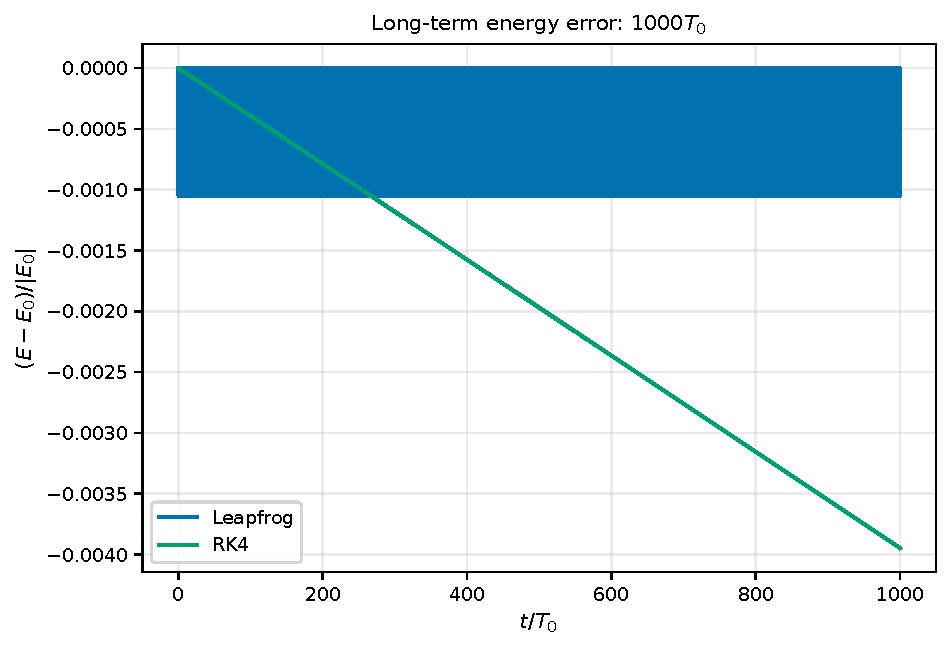
\includegraphics[width=0.68\linewidth]{ch03_long_term_energy.pdf}
\caption{$\Delta t=T_0/50$ で $1000T_0$ まで積分した符号付き相対エネルギー誤差。リープフロッグ法はほぼ一定の範囲で振動し、RK4 には負の方向への長期的なずれが見られる。多数の振動が重なるため、リープフロッグ法の曲線は帯状に見える。}
\label{fig:ch3-long-term}
\end{figure}

表\ref{tab:ch3-long-energy-max}では、リープフロッグ法の最大誤差は最初の $20T_0$ で約 $\chthreeLongEarlyMaxLeapfrog$ に達し、その後もほとんど増えない。
一方、RK4 の誤差は初めは小さいが、時間とともに増加する。
$20T_0$ までの最大誤差は RK4 の方が小さく、$1000T_0$ までではリープフロッグ法の方が小さい。
ただし、大小が入れ替わる時刻は時間刻みに強く依存する。
例えば $\Delta t=T_0/100$ では、$1000T_0$ まで積分しても RK4 の最大誤差の方が小さい。
誤差の大小を比較するときは、時間刻みと積分時間を必ず併記する必要がある。

リープフロッグ法は2次精度だが、時間に依存しない保存力による滑らかな束縛軌道を、十分小さい固定時間刻みで積分すると、エネルギー誤差が一方向に蓄積しにくい性質を持つ\cite{matsumoto}。
これは、物理的エネルギーを各ステップで厳密に保存するという意味ではない。
一方、RK4 が4次精度であることは、固定した終端時刻で時間刻みを小さくしたときの誤差の減少を表す。
収束次数と長時間の保存量の振る舞いは別の性質なので、必要な精度、積分時間、計算コストに応じて方法を選ぶことが重要である。

\begin{topicblock}{リープフロッグ法とシンプレクティック性}
リープフロッグ法の長時間挙動を理解する背景には、保存力による運動が持つ構造がある。
位置と速度を組にした状態を表す空間を\textbf{位相空間}と呼ぶ。
本章のような保存力による運動は、Hamilton 系と呼ばれる枠組みで記述できる。
この系に備わる位相空間の構造を離散的な時間更新でも保つ方法が、\textbf{シンプレクティック積分法（symplectic integrator）}であり、固定時間刻みのリープフロッグ法はその一例である。

この性質は、エネルギーを各ステップで厳密に保存することや、任意の時間刻みで安定に計算できることとは異なる。
精度の次数だけとも区別する必要がある。
実際の $N$ 体計算や SPH 計算では、粒子の状態に応じた\textbf{可変時間刻み（adaptive timestep）}や、
粒子ごとに異なる時間刻み（\textbf{独立時間刻み; individual timestep}）を用いる場合がある。
その場合、本章の共通の固定時間刻みで見た長時間の保存性はそのままでは保証されず、時間刻みの決め方と更新手順を組み合わせた検証が必要になる。

理論的背景は Notebook 3 の補足と松本ほか §9.6\cite{matsumoto}を参照する。
\end{topicblock}


\begin{topicblock}{宇宙流体計算の時間積分：RK2 と RK3}
本章で扱った時間積分は、星の軌道計算だけでなく、空間を離散化した流体の方程式にも用いられる。
例えば有限体積法では、密度・運動量密度・エネルギー密度などのセル平均値を持たせる。
全セルのこれらの量をまとめたベクトルを $\boldsymbol{U}$ とすると、空間方向を離散化した後の時間発展は
\begin{equation}
 \frac{d\boldsymbol{U}}{dt}=\boldsymbol{f}(\boldsymbol{U})
\label{eq:ch3-hydro-ode}
\end{equation}
と書ける。ここでは、右辺が時刻に明示的に依存しない場合を考える。
$\boldsymbol{f}(\boldsymbol{U})$ は、現在の状態からセル境界を通る流束や重力などの効果を評価し、各セルの時間変化率を計算する関数である。
式\eqref{eq:ch3-first-order}と同じ形なので、常微分方程式の時間積分法を適用できる。

格子法の宇宙流体計算では、2次や3次の Runge--Kutta 法も用いられる\cite{fujii2020,matsumoto}。
ここでは、その具体例として2段2次の RK2 と3段3次の RK3 を示す。
$\boldsymbol{U}^n$ は時刻 $t_n$ の数値状態を表し、上付きの $(1)$、$(2)$ は計算途中の補助状態を表す。

2次精度の Heun 法（RK2）は、
\begin{align*}
 \boldsymbol{U}^{(1)}&=\boldsymbol{U}^n+\Delta t\,\boldsymbol{f}(\boldsymbol{U}^n),\\
 \boldsymbol{U}^{n+1}&=\frac12\boldsymbol{U}^n+\frac12\left[\boldsymbol{U}^{(1)}+\Delta t\,\boldsymbol{f}(\boldsymbol{U}^{(1)})\right]
\end{align*}
と書ける。
最初に Euler 法で予測値 $\boldsymbol{U}^{(1)}$ を求め、その予測値でも時間変化率を評価する。
2行目に1行目を代入すると、始点と予測した終点での変化率を平均して更新する式になる。

代表的な3次精度の公式（RK3）では、最初の予測値 $\boldsymbol{U}^{(1)}$ は上の Heun 法と共通である。
その後、次の2段で更新する。
\begin{align*}
 \boldsymbol{U}^{(2)}&=\frac34\boldsymbol{U}^n+\frac14\left[\boldsymbol{U}^{(1)}+\Delta t\,\boldsymbol{f}(\boldsymbol{U}^{(1)})\right],\\
 \boldsymbol{U}^{n+1}&=\frac13\boldsymbol{U}^n+\frac23\left[\boldsymbol{U}^{(2)}+\Delta t\,\boldsymbol{f}(\boldsymbol{U}^{(2)})\right].
\end{align*}
ここで示した RK2 では2回、RK3 では3回、右辺の関数を評価する。
いずれも、Euler 法による予測と既知の状態との重み付き平均を組み合わせた更新として読める。

SPH 法へ拡張して速度依存の力や散逸を扱う場合には、本章の保存力に対するリープフロッグ法の保存性はそのままでは保証されない。
RK2・RK3 でも、空間離散化と組み合わせた時間刻みの制約を満たす必要がある。
詳しくは藤井・立川\cite{fujii2020}、松本ほか\cite{matsumoto}を参照すること。
\end{topicblock}

% =====================================================================
